\documentclass[tikz,border=10pt]{standalone}
\usetikzlibrary{calc}
\begin{document}
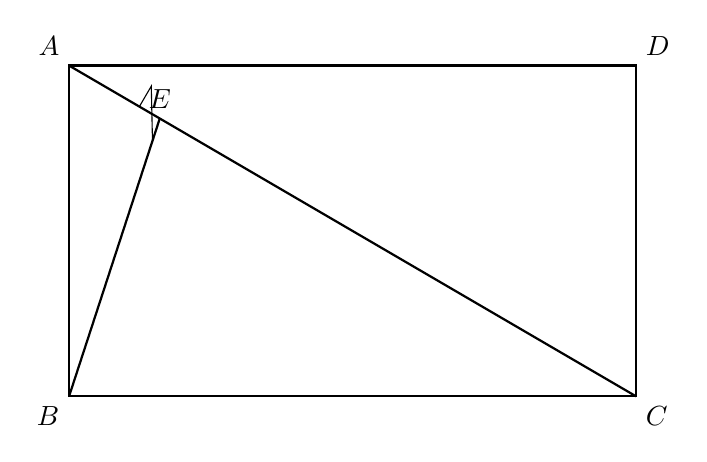
\begin{tikzpicture}[scale=1.2]
\coordinate (A) at (0,3.5);
\coordinate (B) at (0,0);
\coordinate (C) at (6,0);
\coordinate (D) at (6,3.5);
\coordinate (E) at ($(A)!0.16!(C)$);
\draw[thick] (A) -- (B) -- (C) -- (D) -- cycle;
\draw[thick] (A) -- (C);
\draw[thick] (B) -- (E);
% right angle mark at E between EA and EB
\draw ($(E)!{0.25cm}!(A)$) -- ($($(E)!{0.25cm}!(A)$)!{0.25cm}!90:(E)$) -- ($(E)!{0.25cm}!(B)$);
\node[above left] at (A) {$A$};
\node[below left] at (B) {$B$};
\node[below right] at (C) {$C$};
\node[above right] at (D) {$D$};
\node[above] at (E) {$E$};
\end{tikzpicture}
\end{document}
